\chapter{Signal Simulation}
Because the signal process for \dbrem occurs between outgoing particles from the collision and nuclei within the detector, it must be built into the \gf simulation of the detector reponse instead of directly imported as an initial state from an event generator. A custom process was created to accomplish this \cite{Eichlersmith_2023}, and the techniques used therein are described in this chapter. The cross section and kinematics produced by the process are compared to an existing \mg package \cite{madgraph_2014, darkgauge} which provides an accurate implementation of the underlying matrix element based on an input field theory model.
The initial state used for signal simulation is the DY process decaying to two muons, with identical settings to the background DY generation other than the enabled signal process. 

In order to efficiently produce signal events, $\epsilon$ is set to one and the cross section is multiplied by fixed biasing factors for each \aprime mass. 
Additionally, the interaction is only enabled within the HCAL endcap and is disabled after the \aprime is produced to avoid non-physical events with multiple \dbrem interactions that could be caused by the increased interaction probability.
The increased interaction rate biases events towards the center of the detector, as deeper regions see a reduced number of muons due to earlier \dbrem interactions.
This bias is rougly proportional to the fraction of muons undergoing \dbrem squared, so the bias factors are selected to have rates less than 5$\%$. 
A table of the biasing factors used, as well as the corresponding signal rate per incident muon, is presented in \cref{table:dbrem_biasfactors}.
Simulated events that have no \dbrem or do not pass the base event selection are discarded.

\begin{table}[h]
    \centering
    \spacerows{1.2}
    \begin{center}
        \begin{tabular}{@{}l rr@{}}
            \toprule
            \aprime Mass (\SI{}{\giga\eV})& Bias Factor & Interaction Rate\\
            \midrule
            0.2&800&0.22\\
            0.4&1200&0.10\\
            0.6&1600&0.06\\
            0.8&2500&0.04\\
            1.0&3200&0.04\\
            \bottomrule
        \end{tabular}
        \caption{
            Bias factors used in \dbrem generation.
        }
        \label{table:dbrem_biasfactors}
    \end{center}
\end{table}

\section{Technique}
\label{sec:technique}

The physics of \dbrem was implemented in \gf via the creation of an additional physics process class describing the interaction. 
\gf discretizes the simulation of physics into "steps" of time. 
During each step of particle simulation, \gf uses the total cross section all possible physics interactions for that particle to determine which, if any, interactions should occur, then modifies the particle kinematics and generates secondaries as necessary. 
In this implementation, the cross section is calculated by performing a numerical integration of the \ww approximation.
The relative accuracy of this approximation for the energy range used in CMS is shown in \cref{fig:mu_xsec}.
The result depends on the mass of the \aprime,  the energy of the incident muon, and the material it passes through. 

While the total cross section given by the numerical integral of the \ww approximation is effective for the purposes of this analysis, it was found that the differential result it produces has significant deviations from \mg, particularly in the limits of large angular scatters and high \aprime energy. 
The kinematics of the interaction are further complicated by the presence of the scattered nucleus. 
The \ww approximation produces differential distributions for the kinematics of the outgoing \aprime, but the kinematics of the scattered muon determine what is visible in the detector. 
As the nucleus can carry momentum comparable to the muon, reconstructing the outgoing muon without including the momentum carried by nucleus produces significantly different distributions in the recoil muon momentum and angle. 
To circumvent these issues the simulation does not construct outgoing muons by sampling from the differential \ww cross section, but instead scales existing \mg events to the desired incident muon energy. 

\begin{figure}[!htbp]
    \centering
    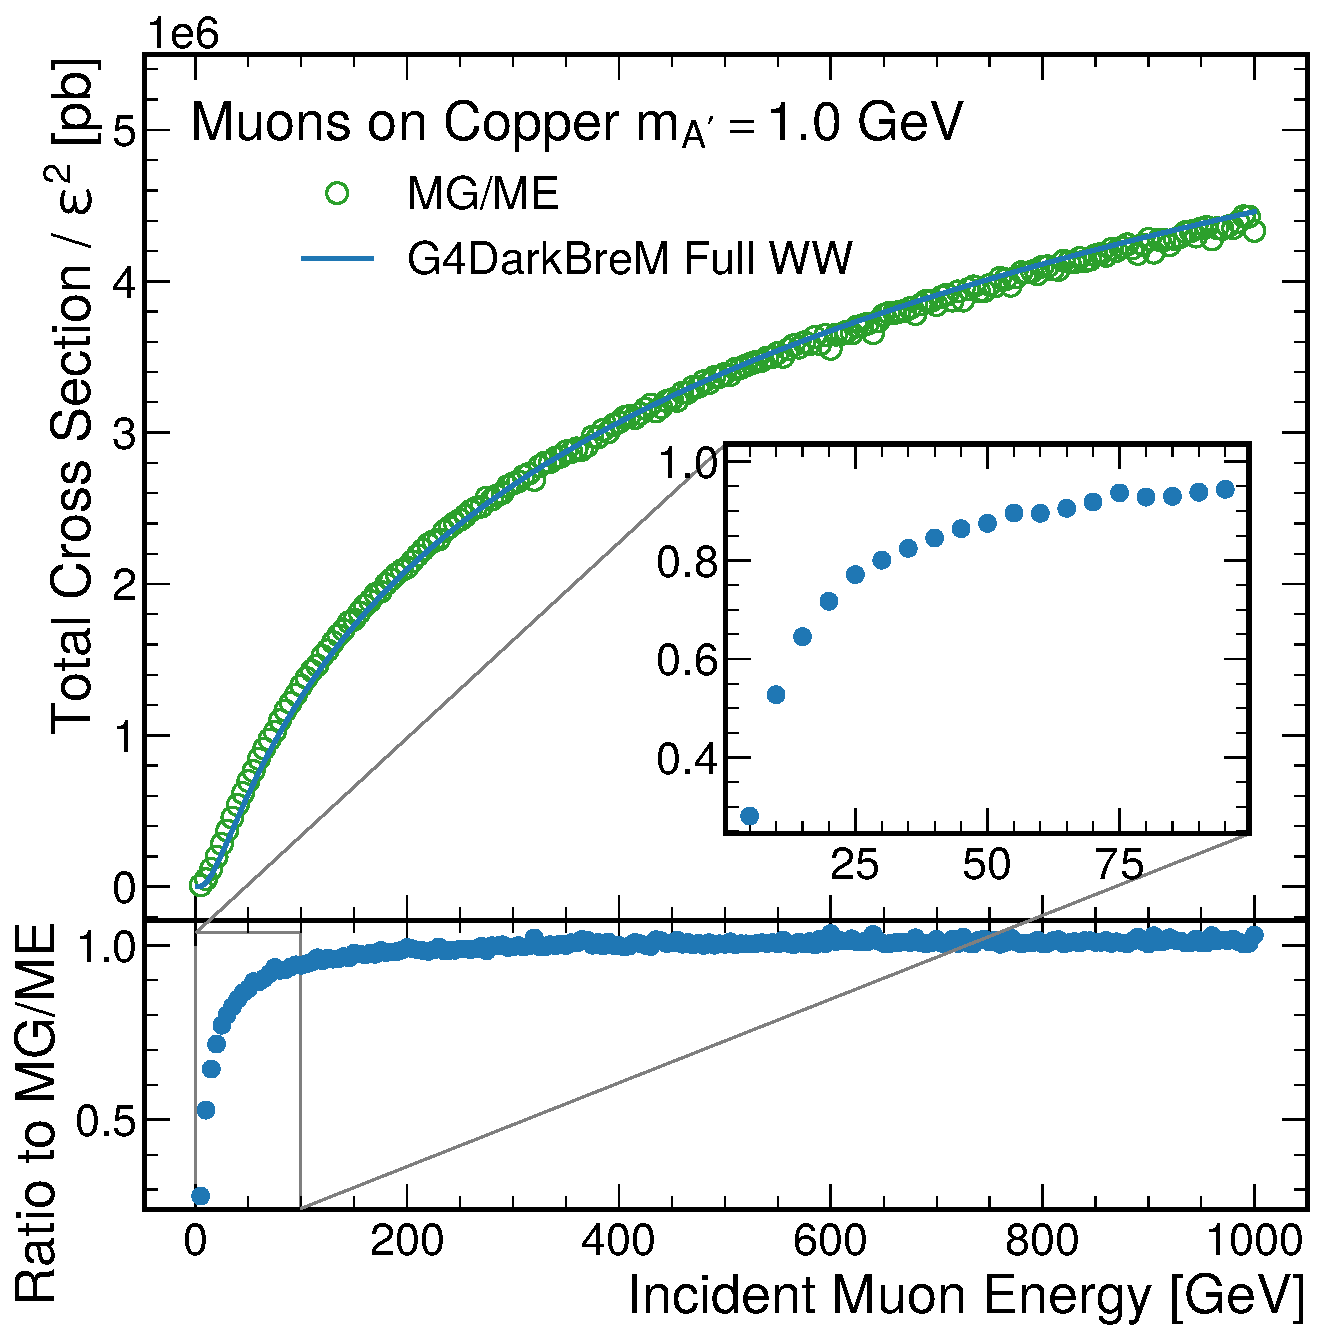
\includegraphics[width=\textwidth]{figures/mu_xsec.pdf}
    \caption[
        The \dbrem cross section.
    ]{
        The total \dbrem cross section for muons incident on copper. 
    }
    \label{fig:mu_xsec}
\end{figure}

Through study of \mg events produced over a range of incident muon energies, two variables with distributions that vary slowly with incident energy were identified: the fraction of the incident kinetic energy imparted to the scattered muon and the transverse momentum of that muon with respect to the incident particle (\cref{fig:efrac_pt}). 
Because of this slow variation with incident energy, we can sample these variables from a set of previously simulated \mg events at a ``nearby'' energy and rescale them to the desired initial energy without introducing large error. 
The two variables are correlated, so they must be sampled together. 
The scaling from a sampled \mg incident energy to the actual \gf incident energy has been found effective over a wide range; nevertheless, the differences become more pronounced as the relative distance between the sampled and true incident energies increases.
The impact of these variations is limited by using fine-binned energies in the sampled \mg libraries, and a systematic uncertainty is assessed by scaling each event to the second-nearest available energy to account for these potential differences. 

\begin{figure}[!htbp]
    \centering
    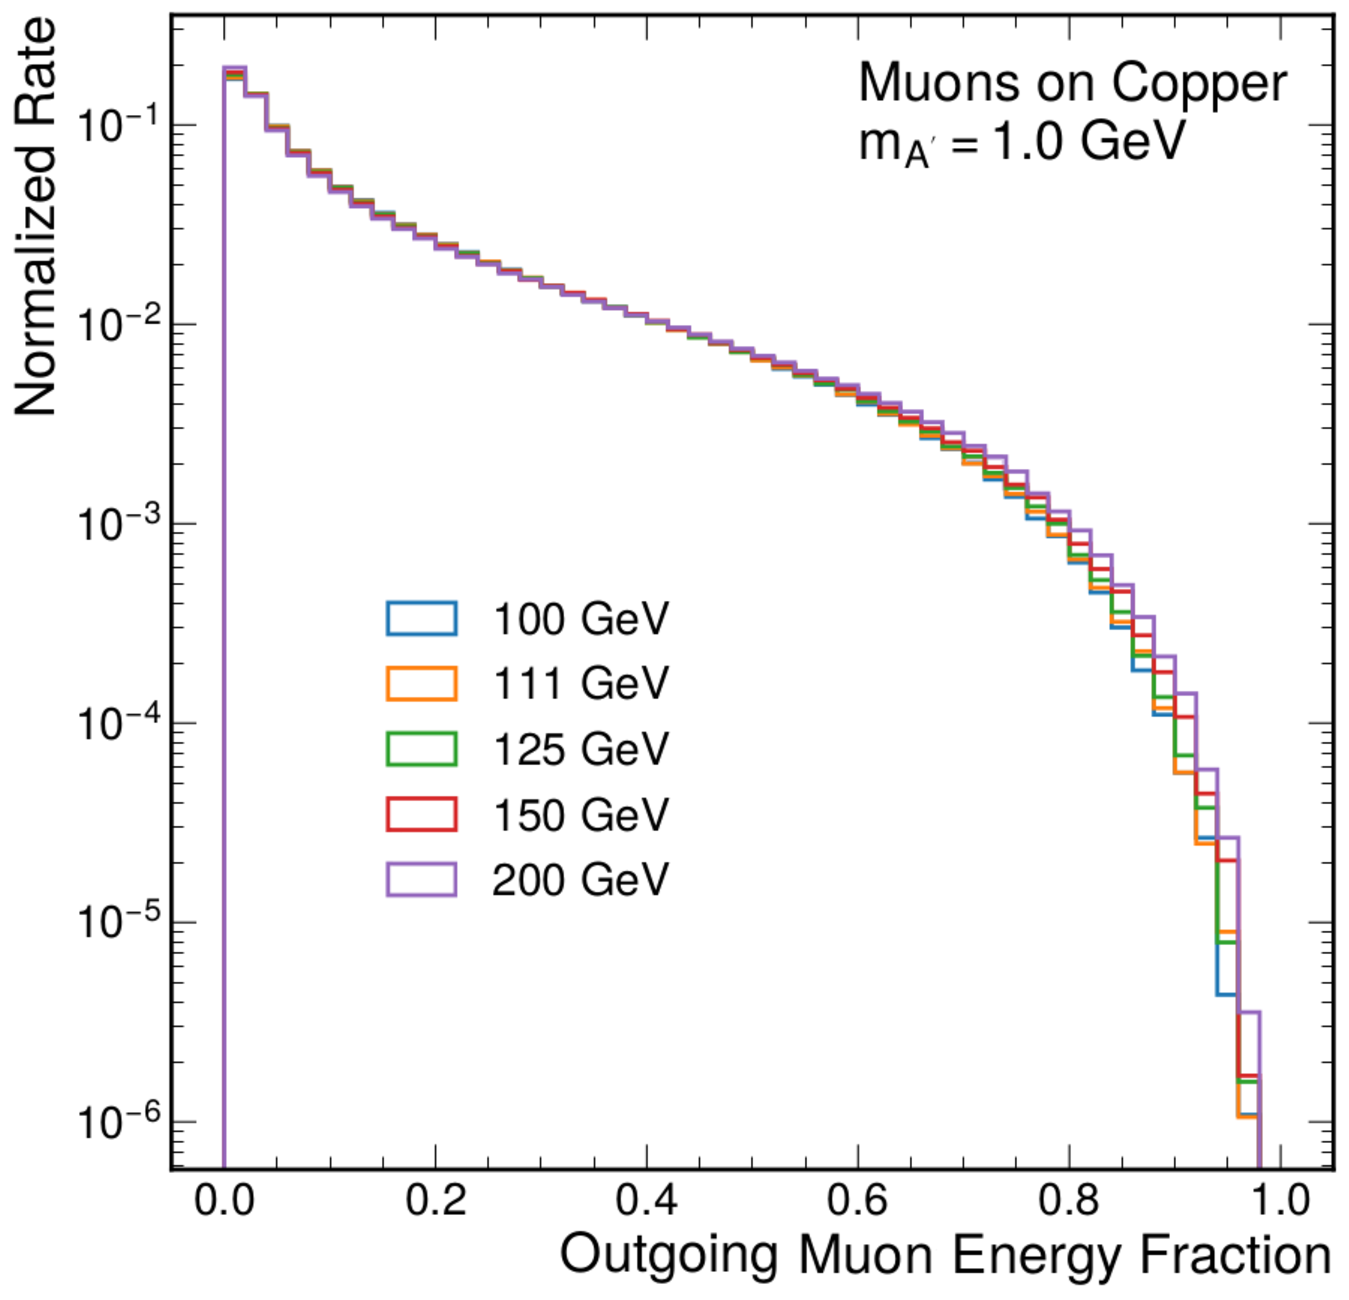
\includegraphics[width=0.45\textwidth]{figures/muon_energy_comp_efrac.pdf}
    \hspace{0.01\textwidth}
    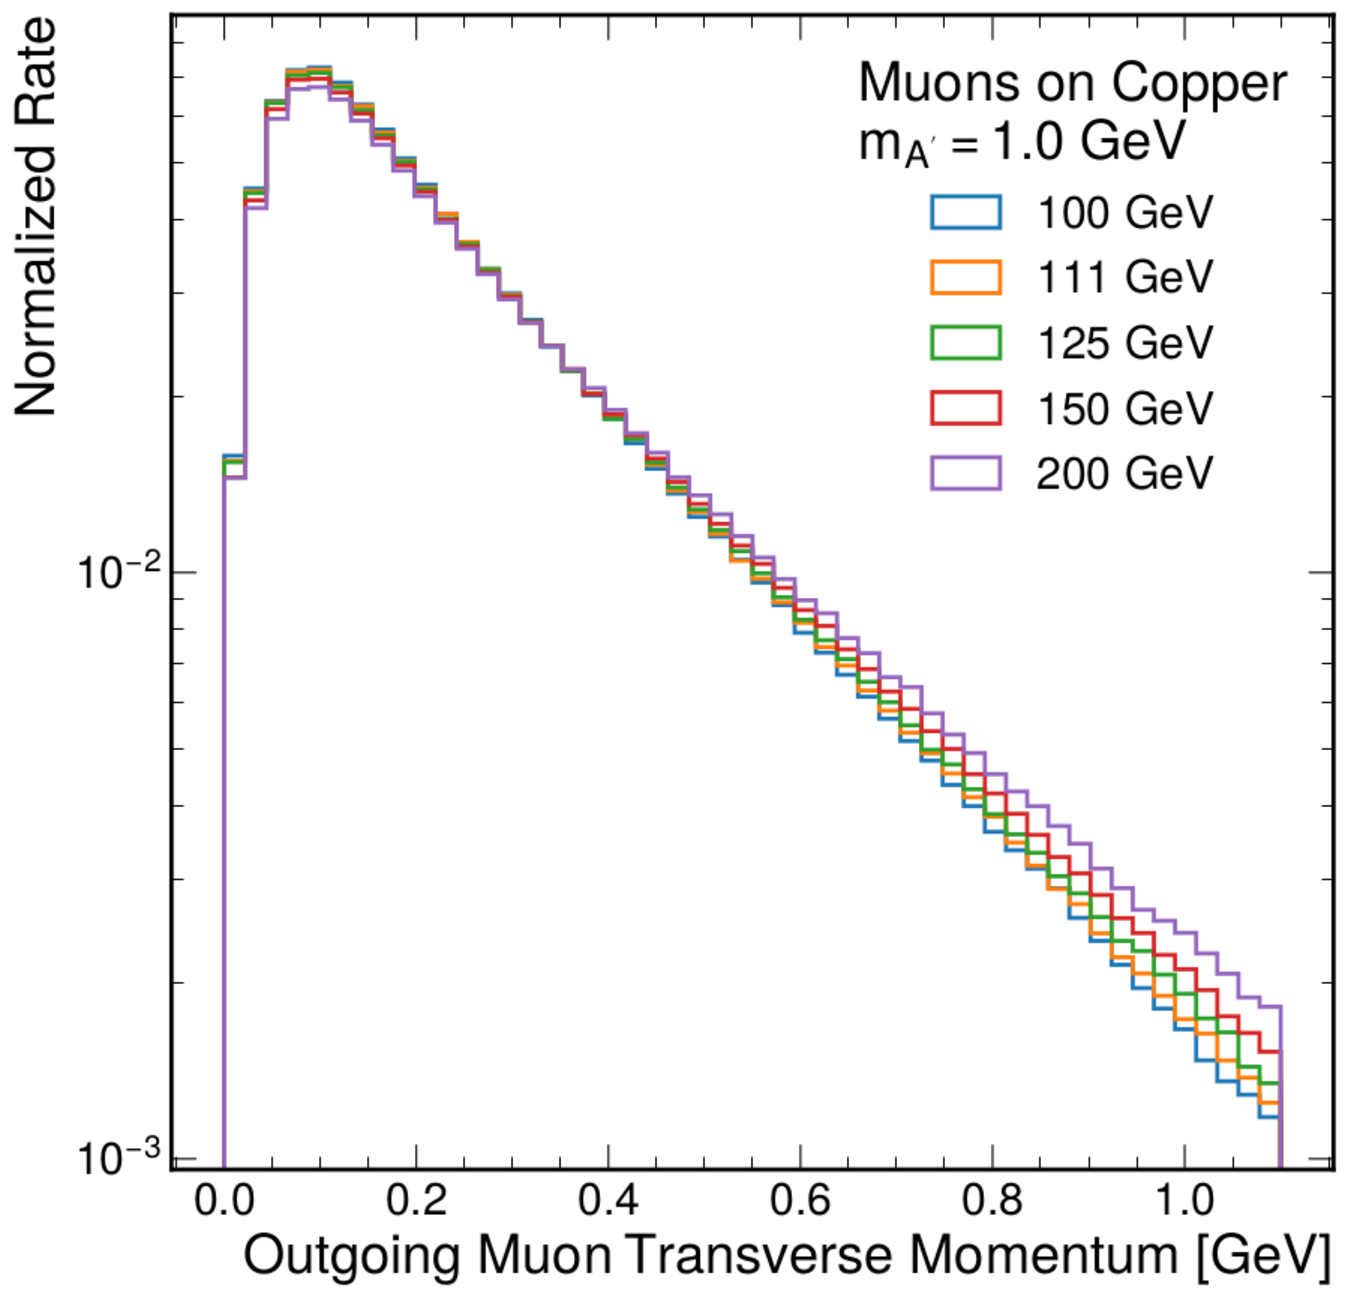
\includegraphics[width=0.45\textwidth]{figures/muon_energy_comp_pt.pdf}
    \caption[
        Sampling variables used for \dbrem simulation.
    ]{
        The outgoing muon energy fraction (left) and transverse (right) for muons incident on copper. Despite large shifts in the incident muon energy, the two distributions of the two variables remain relatively constant. 
    }
    \label{fig:efrac_pt}
\end{figure}

When \gf determines that a \dbrem event should occur in the simulation, the process selects a random event from the nearest available muon energy and target material in the loaded \mg library. 
\gf then creates a muon with the same transverse momentum as the sampled event and scales the outgoing kinetic energy to match the fraction of incident kinetic energy of the sampled muon, then randomly selects an azimuthal angle with respect to the initial muon momentum. 
In the rare case where the rescaled total energy of the deflected muon would be smaller than the selected transverse momentum, alternate events are sampled until one is found with final energy larger than its transverse momentum. 

The simulation assumes that the scattered nucleus does not receive sufficient momentum to produce an observable signal in the detector; therefore, no \gf particle for the scattered nucleus is created and, as a result, energy and momentum cannot be precisely conserved using only the \aprime and scattered muon. 
In searches with visible \aprime and muon signatures this effect would introduce un-accounted for correlations between the secondaries, but with an invisible \aprime only the muon requires correct kinematics and an arbitrary outgoing \aprime can be produced.  
The simulation produces an \aprime using only conservation of momentum so that the incident muon can be reconstructed from simulation-level information about the \aprime and the scattered muon.
No physics processes are been implemented for the emitted \aprime to ensure that it remains invisible to the detector.

The kinematics of the outgoing muon depend weakly on the composition of the target material.
The core assumptions of the scaling technique, slow variation of transverse momentum and outgoing energy fraction spectra with respect to incident energy, are found to remain valid across a wide range of target materials while the underlying distributions of those variables have small dependences on the material type (\cref{fig:dbrem_material}).
Because the kinematics have small variation with scattering material, all \dbrem interactions in this analysis are scaled from samples produced with a copper target, which is the most frequent \dbrem initiating material in the CMS HCAL endcap (See Table \ref{table:dbrem_material}).   

\begin{figure}[!htbp]
    \centering
    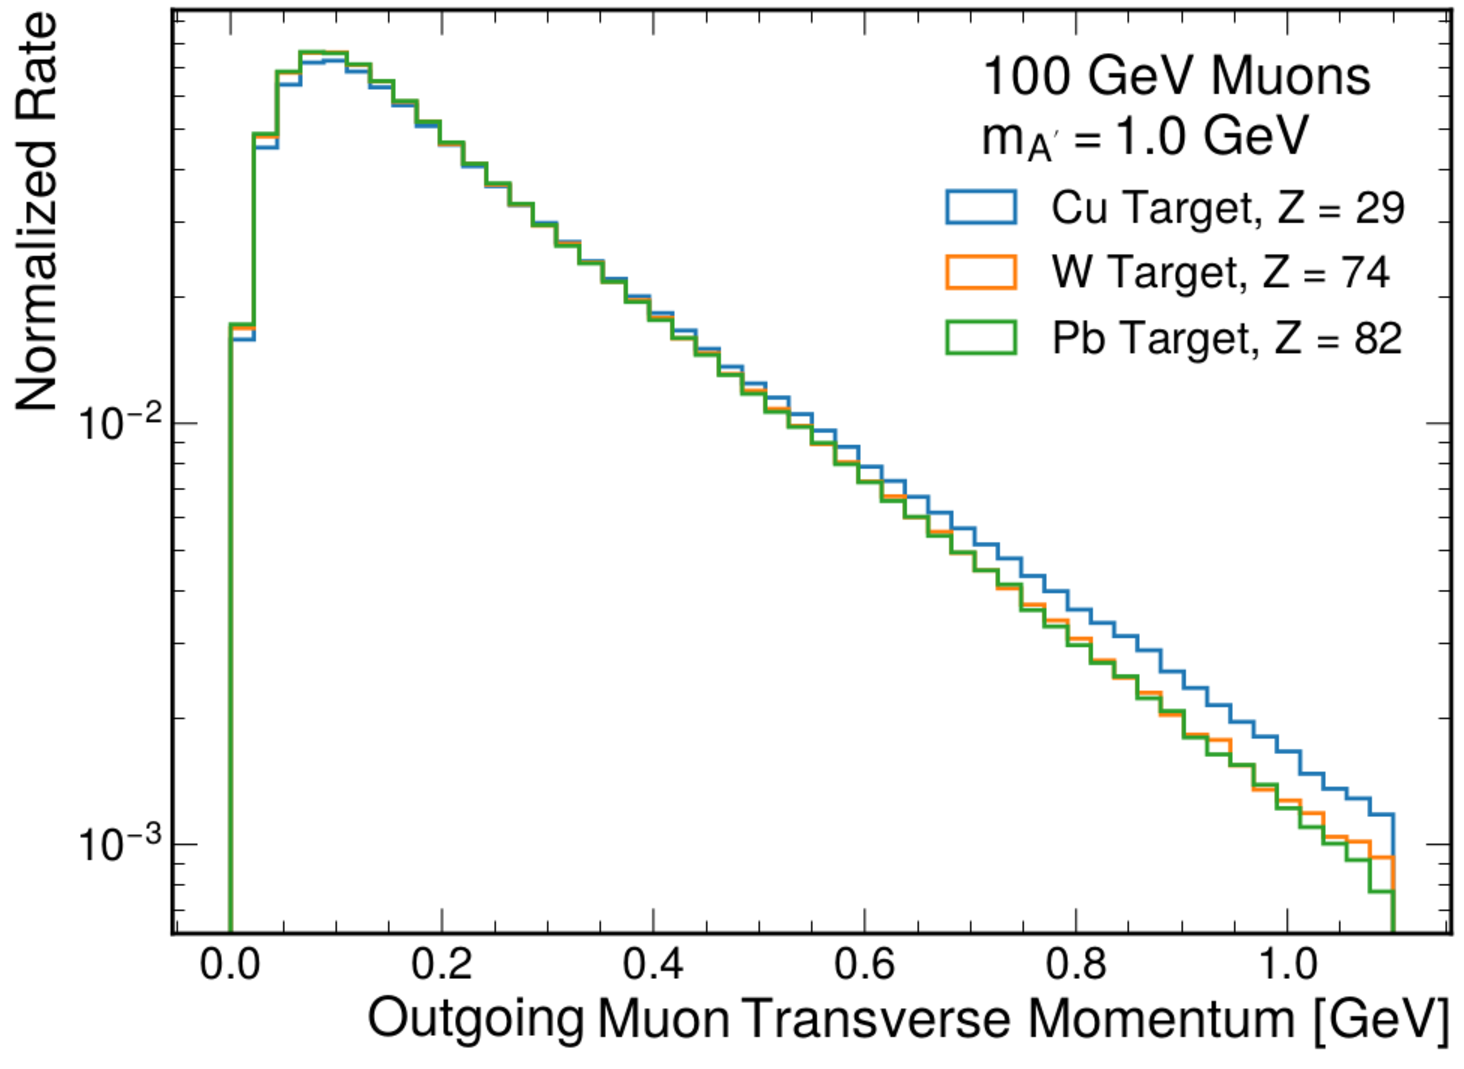
\includegraphics[width=0.45\textwidth]{figures/muon_material_comp_pt.pdf}
    \hspace{0.01\textwidth}
    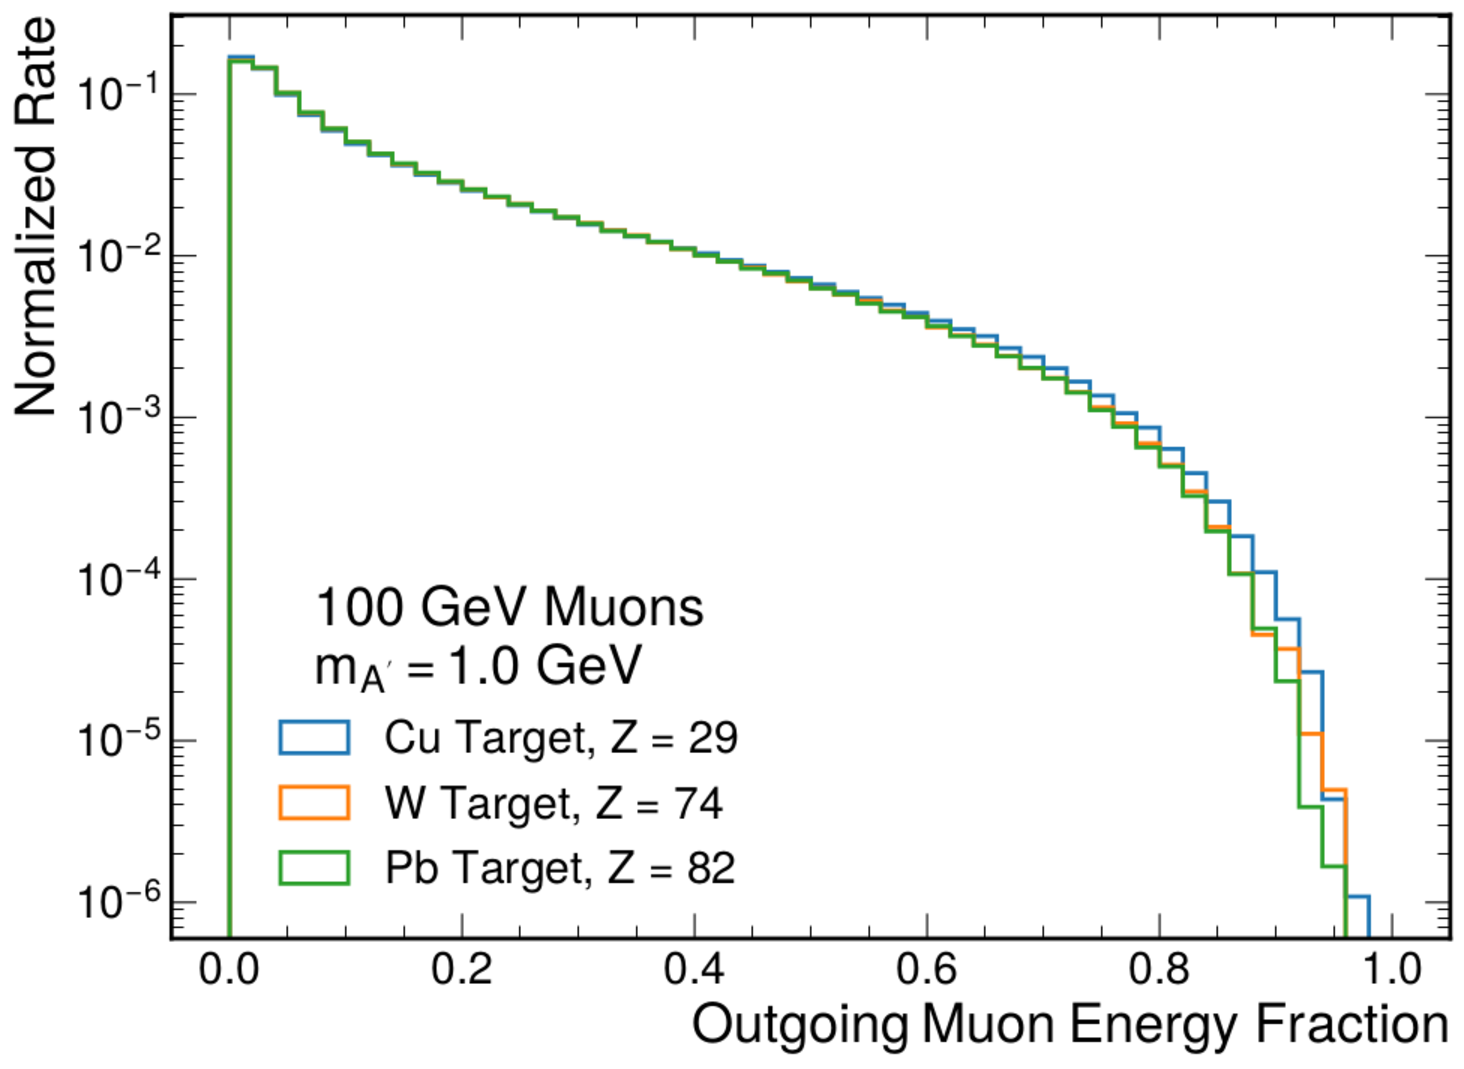
\includegraphics[width=0.45\textwidth]{figures/muon_material_comp_efrac.pdf}
    \caption[
        Material dependence of \dbrem kinematics.
    ]{
        The outgoing muon transverse momentum (left) and energy fraction (right) for muons incident on copper, lead, and tungsten. While materials close in Z have smaller relative shifts, the overall distributions are similar even with large changes in material. 
    }
    \label{fig:dbrem_material}
\end{figure}

\begin{table}[h]
    \centering
    \spacerows{1.2}
    \begin{center}
        \begin{tabular}{@{}l rr@{}}
            \toprule
            Material & 0.2 GeV & 1.5 GeV\\
            \midrule
            Copper&0.69&0.67\\
            Zinc&0.29&0.29\\
            Iron&0.02&0.03\\
            Chromium&0.004&0.01\\
            Carbon&0.002&0.003\\
            Nickel&0.001&0.005\\
            Hydrogen&0.001&0.0004\\
            Manganese&0.0004&0.0001\\
            Oxygen&0.0001&1.6$*10^{-5}$\\
            Nitrogen&3$*10^{-6}$&0\\
            \bottomrule
        \end{tabular}
        \caption{
            The fraction of \dbrem events initiated by detector material.
        }
        \label{table:dbrem_material}
    \end{center}
\end{table}
    
\section{Validation}
\label{sec:validation}

Comparing the recoil muon kinematics produced using this scaling procedure to a sample of \mg events at the target incident energy shows that this procedure does not significantly distort the distributions (\cref{fig:dbrem_validation}).
Moreover, these figures show that the scaling procedure more-closely resembles the ``true" \mg distribution the smaller the scaling distance is.

The outgoing muon angle is less well reconstructed using this procedure; however, the distributions stay within roughly 10\% of the \mg distributions for small scaling distances and scattering angles.
Large muon scattering angles are generally accompanied by very low outgoing energies, producing strongly signal-like events regardless of the outgoing angle. 
This procedure \emph{does not} reconstruct the sign of the outgoing muon's z-momentum, so it is always chosen to be positive. 
Due to the low rate of large scatters and the low outgoing muon energy of these events, the deviations seen above scattering angles of \SI{0.5}{\radian} do not significantly impact the signal efficiency.

\begin{figure}[!htbp]
    \centering
    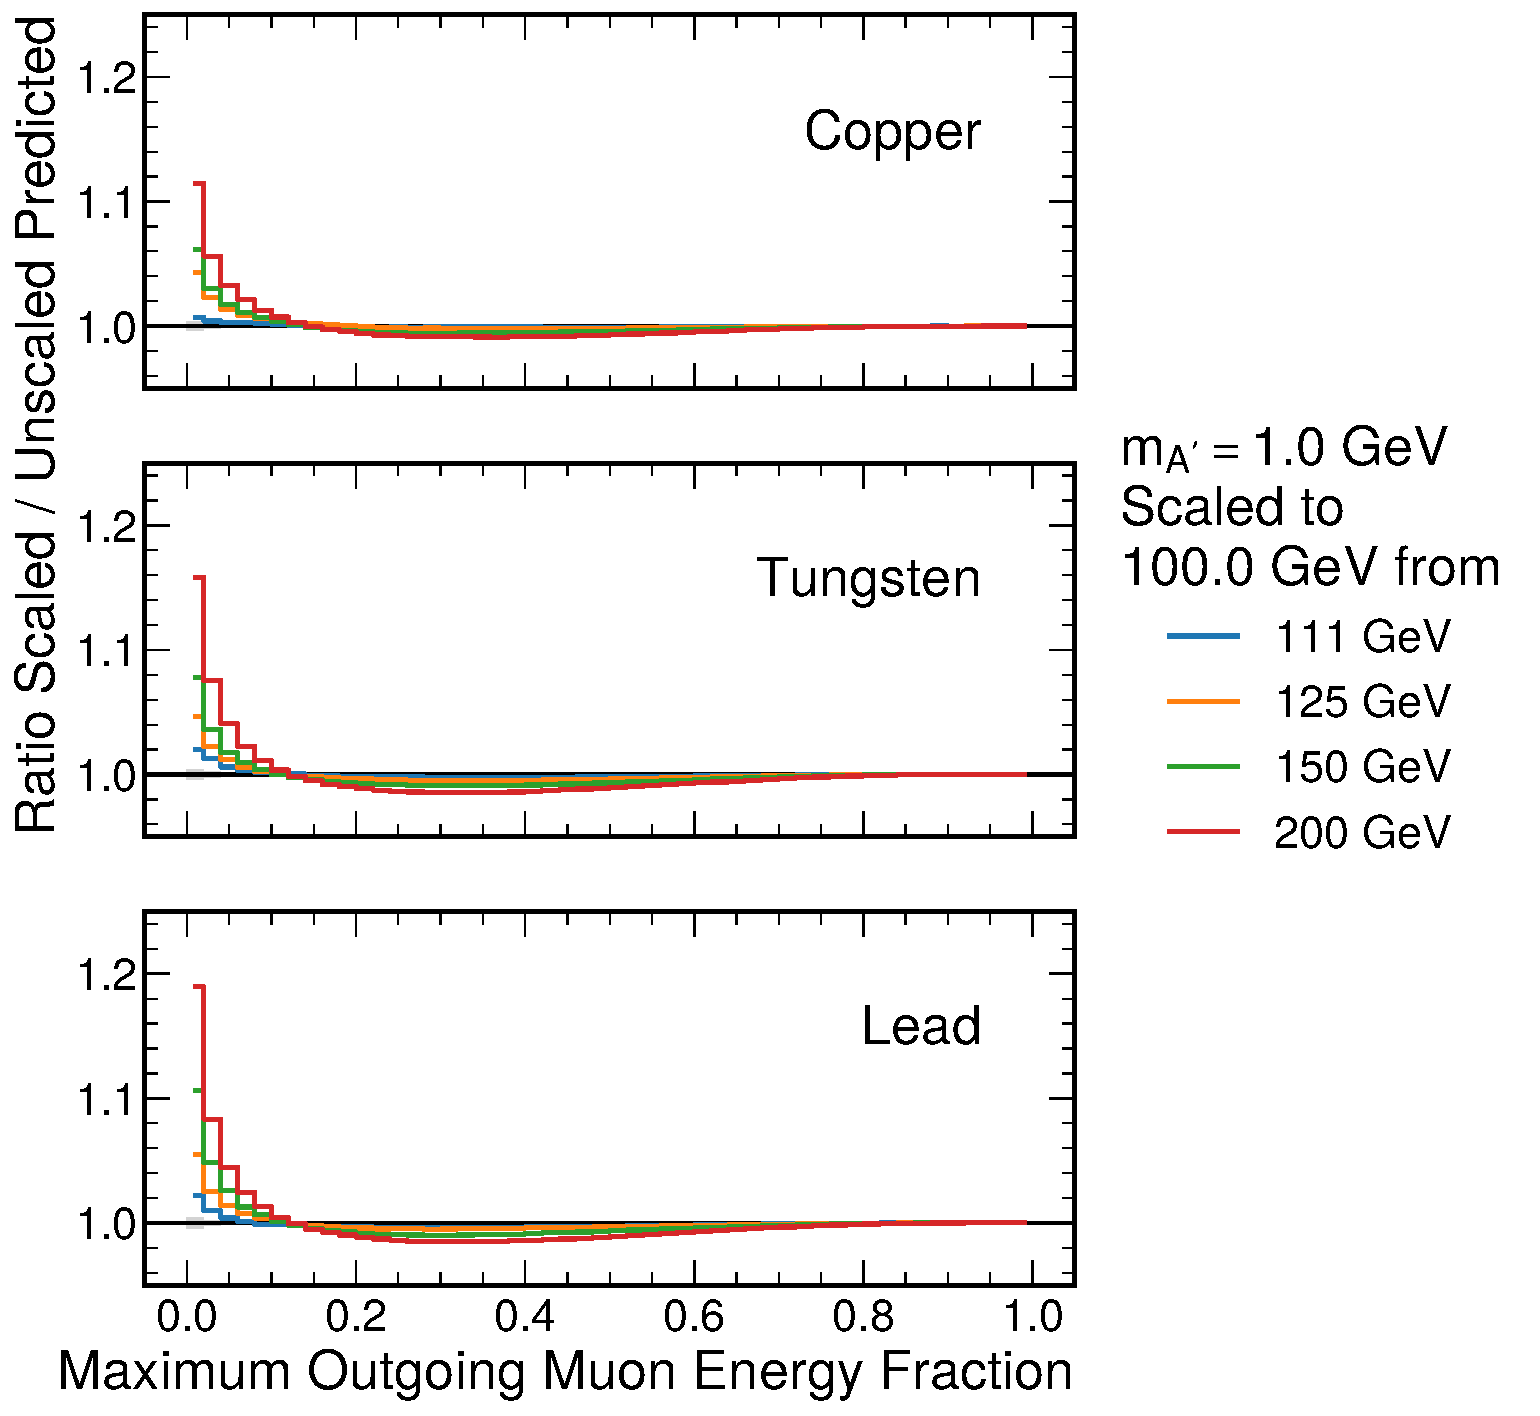
\includegraphics[width=0.45\textwidth]{figures/muon_efrac_cumulative_ratio.pdf}
    \hspace{0.01\textwidth}
    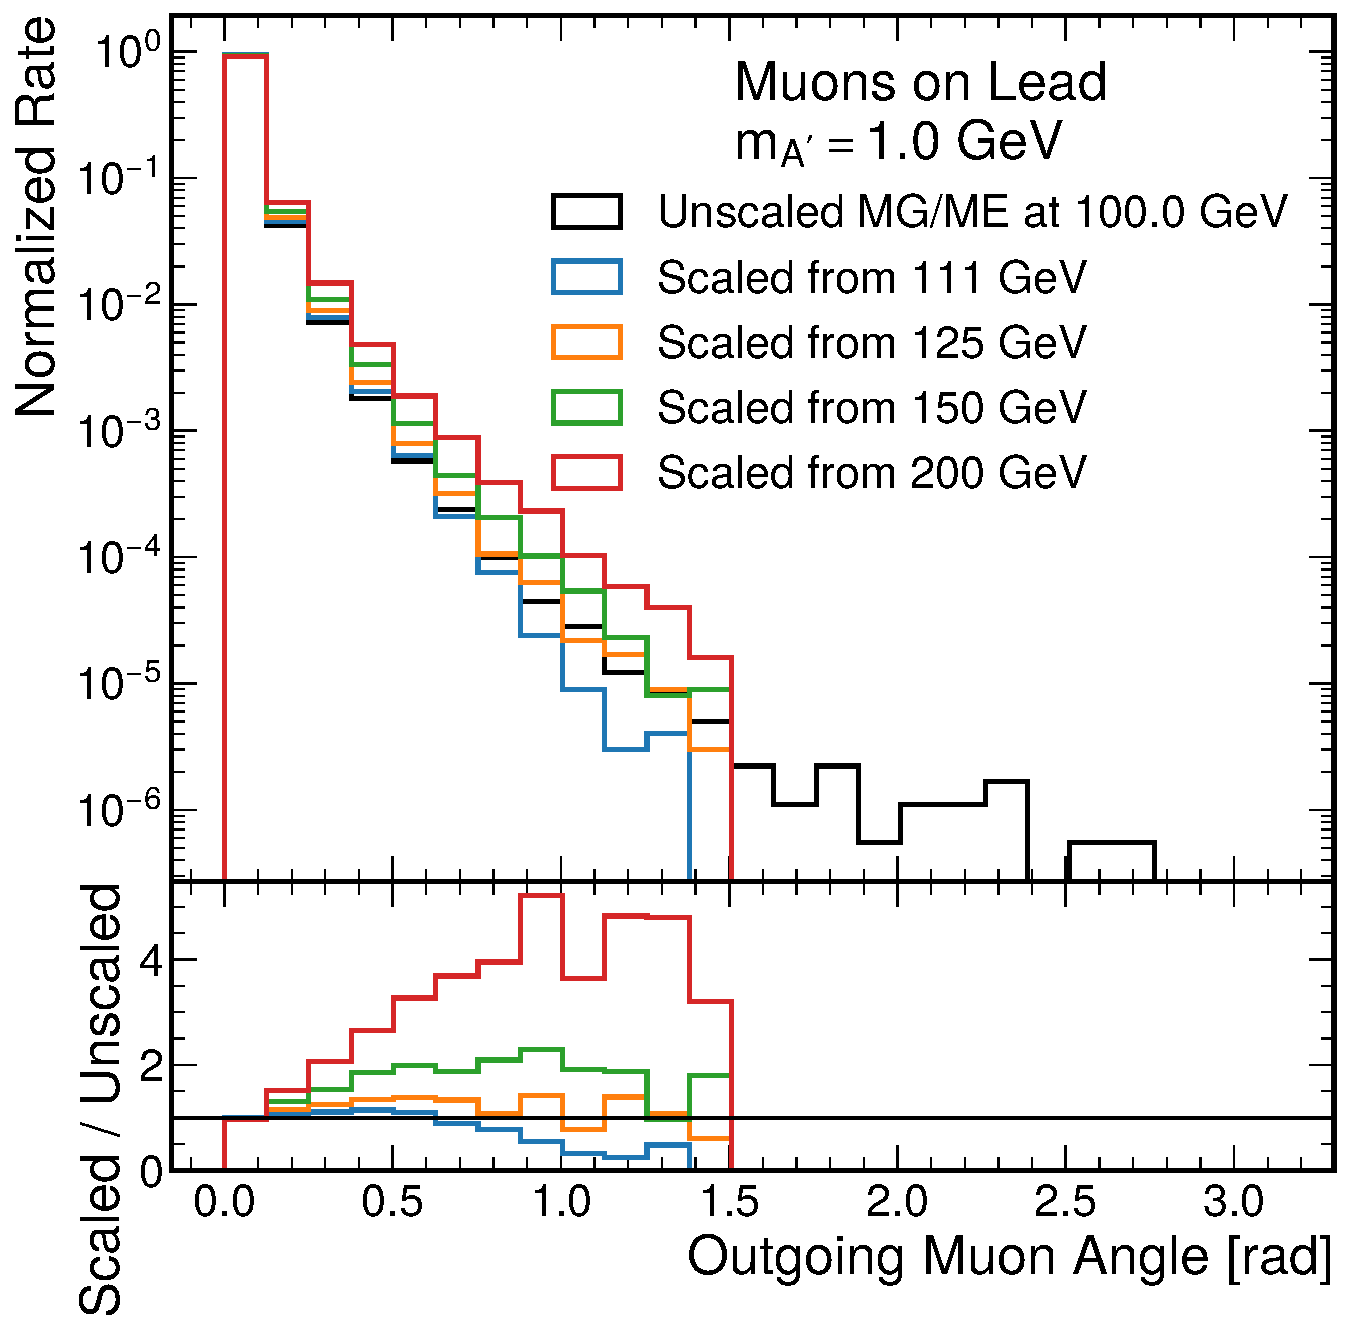
\includegraphics[width=0.45\textwidth]{figures/muon_lead_ang.pdf}
    \caption[
        Validation of simulated \dbrem kinematics.
    ]{
        The outgoing muon energy fraction for various scaling distances in copper, lead, and tungsten (left) and the muon deflection angle (right) for muons incident on lead.
    }
    \label{fig:dbrem_validation}
\end{figure}